\documentclass{article}

\usepackage{graphicx}
\usepackage{tikz}
\usepackage{tikzsymbols}
\usetikzlibrary{calc,patterns,shapes.geometric}
\pagestyle{empty}
\usepackage[margin=0pt]{geometry}
\geometry{papersize={14in,12in}}

\def\centerarc[#1](#2)(#3:#4:#5){\draw[#1] ($(#2)+({#5*cos(#3)},{#5*sin(#3)})$) arc (#3:#4:#5);}

\begin{document}
	\begin{figure}
		\centering
		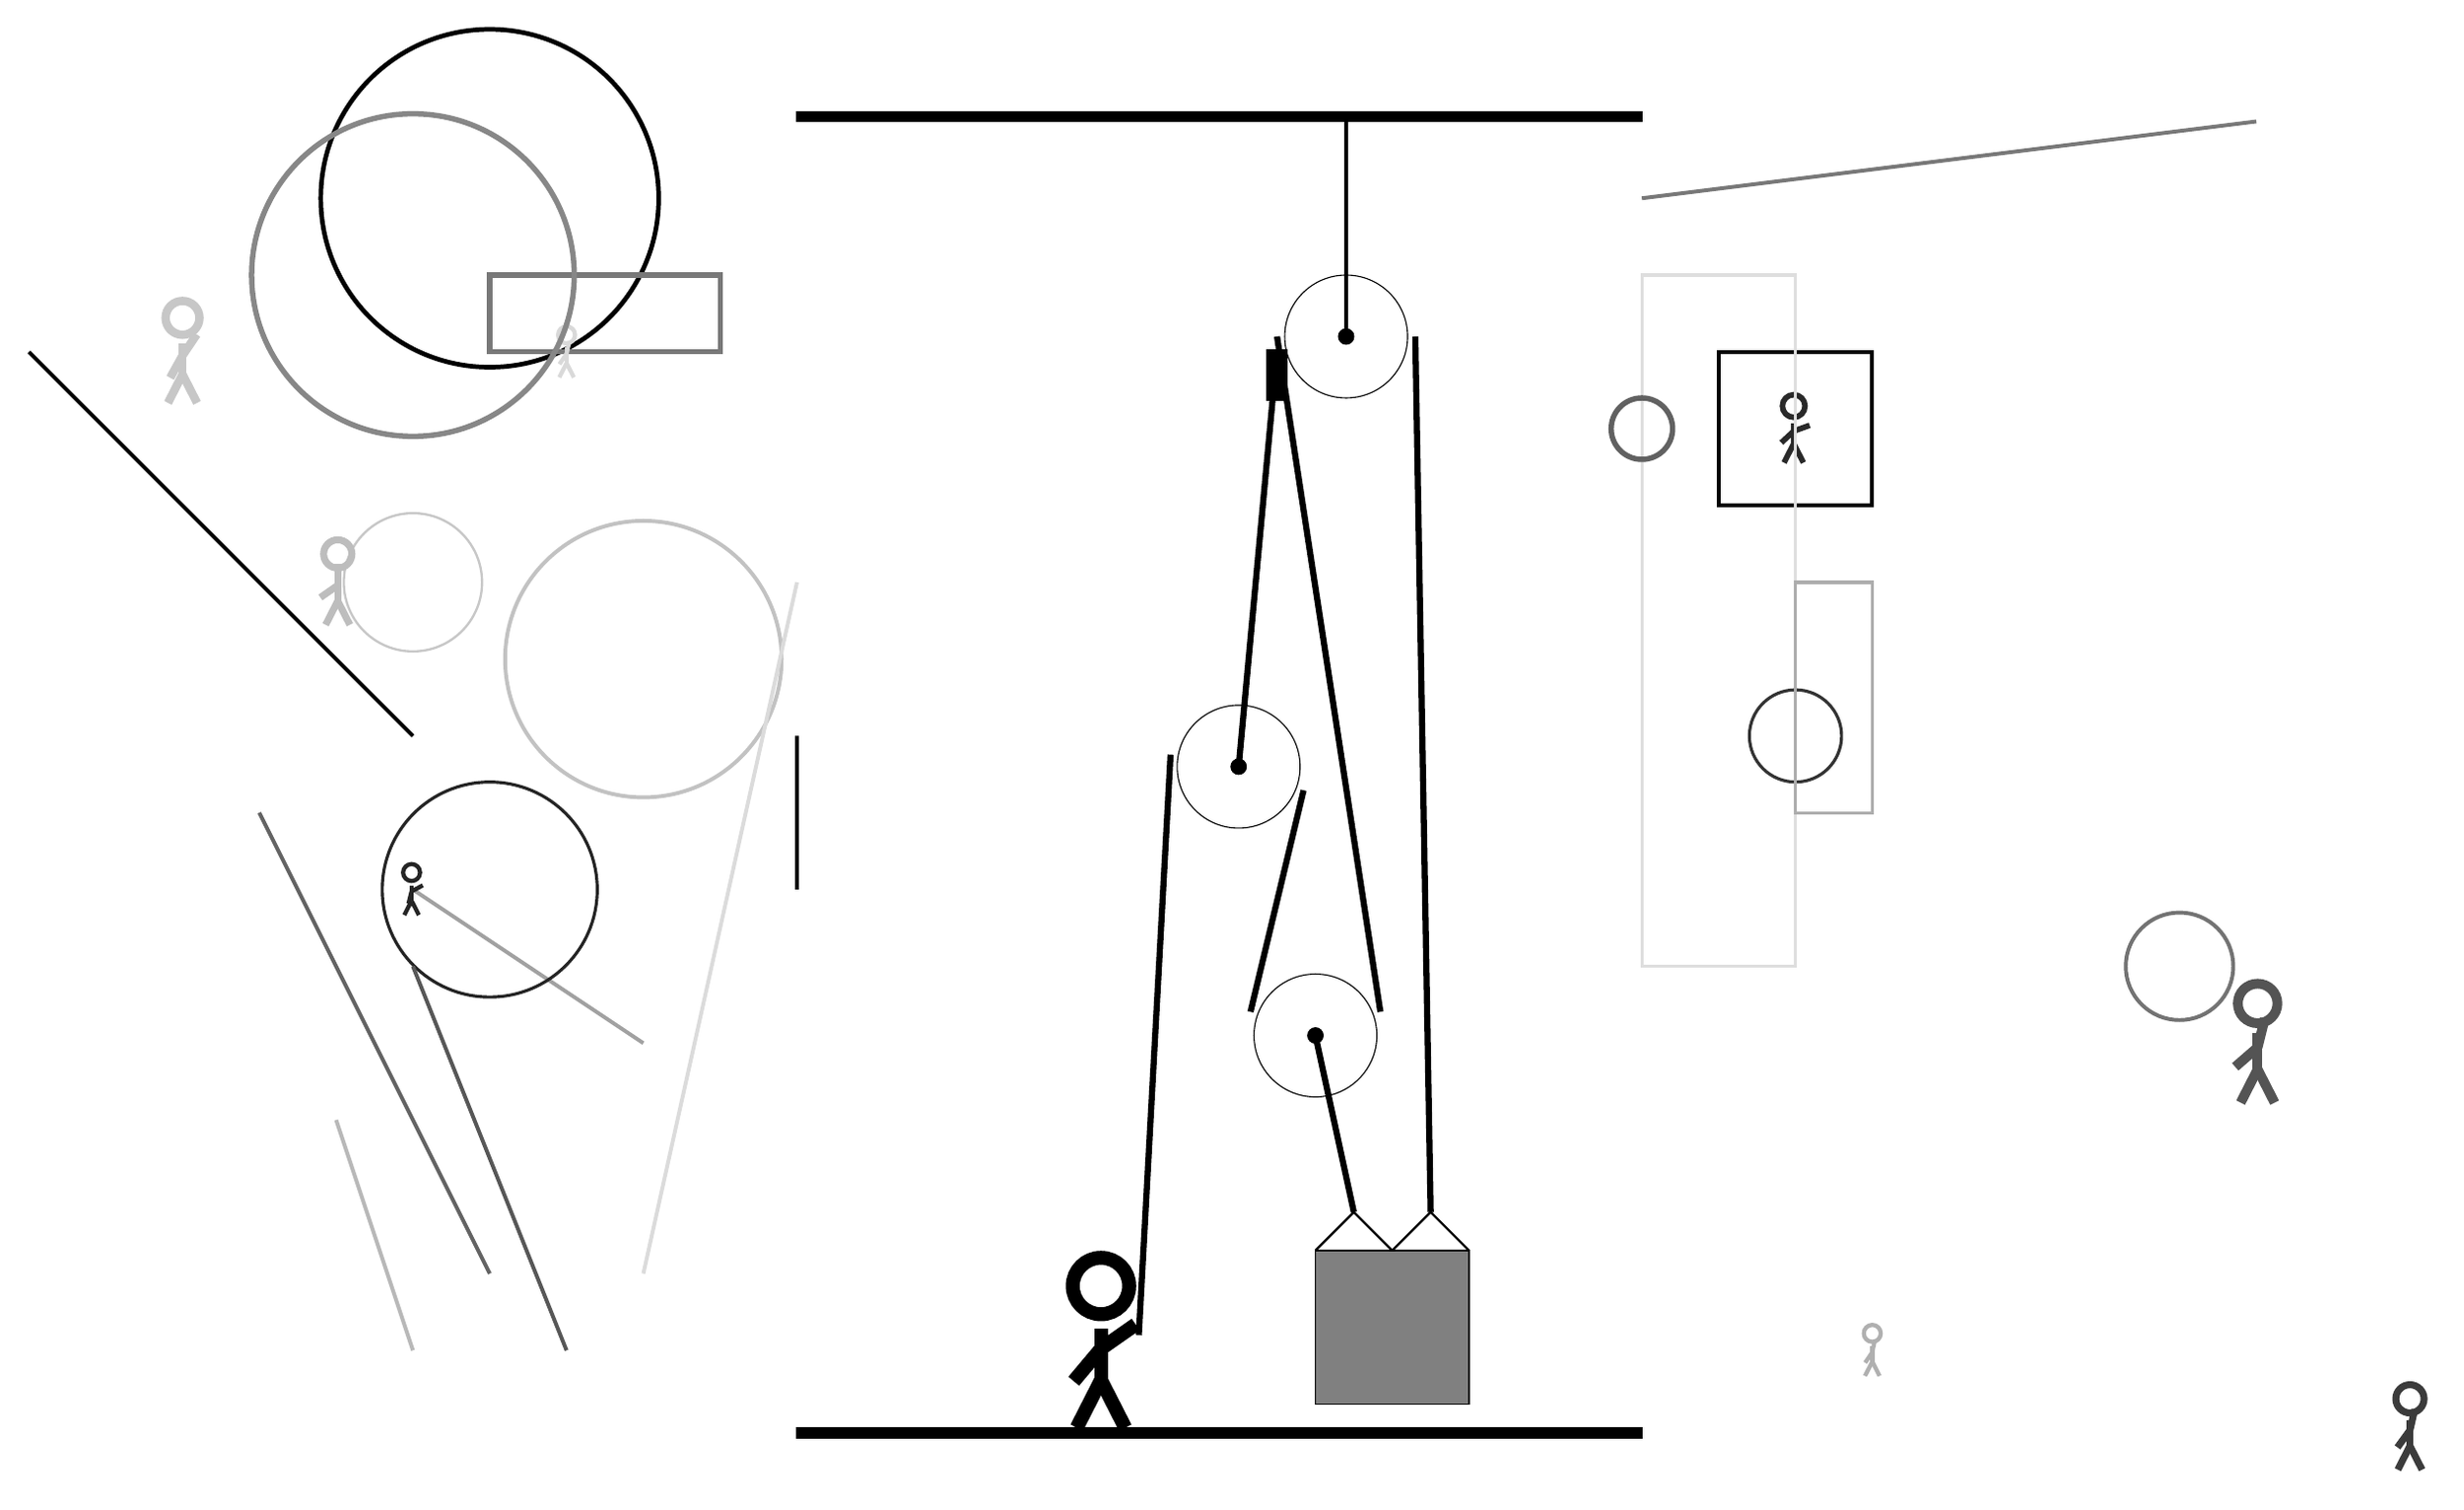
\begin{tikzpicture}
			%%%%% START %%%%%
			
			\draw[fill=black] (-6, 14) rectangle (5, 14.125);
			
			\draw[line width=0.5mm, color=black!99] (6, 11) rectangle (8, 9);
			
			\node[line width=0.6mm, color=black!31] at (8, -2) {\Strichmaxerl[3][56][78]};
			\node[line width=0.2mm, color=black!77] at (15, -3) {\Strichmaxerl[5][54][77]};
			\draw [line width=0.5mm, color=black!24](-8, 7) circle (1.8);
			
			\draw[line width=0.5mm, color=black!37](-8, 2) -- (-11, 4);
			\draw [line width=0.6mm, color=black!100](-10, 13) circle (2.2);
			\node[line width=0.4mm, color=black!84] at (7, 10) {\Strichmaxerl[4][43][20]};
			\draw [line width=0.4mm, color=black!80](7, 6) circle (0.6);
			\draw[line width=0.7mm, color=black!53] (-7, 11) rectangle (-10, 12);
			
			\draw[line width=0.5mm, color=black!100](-11, 6) -- (-16, 11);
			
			\node[line width=0.2mm, color=black!15] at (-9, 11) {\Strichmaxerl[3][56][77]};
			\draw [line width=0.3mm, color=black!22](-11, 8) circle (0.9);
			\draw[line width=0.5mm, color=black!53](5, 13) -- (13, 14);
			
			\draw[line width=0.4mm, color=black!13] (5, 3) rectangle (7, 12);
			\node[line width=0.2mm, color=black!22] at (-14, 11) {\Strichmaxerl[6][61][56]};
			\node[line width=0.7mm, color=black!26] at (-12, 8) {\Strichmaxerl[5][35][90]};
			
			\draw [line width=0.7mm, color=black!62](5, 10) circle (0.4);
			\draw [line width=0.4mm, color=black!86](-10, 4) circle (1.4);
			\draw [line width=0.7mm, color=black!47](-11, 12) circle (2.1);
			\draw[line width=0.5mm, color=black!66](-11, 3) -- (-9, -2);
			\draw[line width=0.4mm, color=black!32] (7, 8) rectangle (8, 5);
			
			\node[line width=0.6mm, color=black!67] at (13, 2) {\Strichmaxerl[7][41][76]};
			\draw [line width=0.5mm, color=black!55](12, 3) circle (0.7);
			\draw[line width=0.6mm, color=black!97] (-6, 6) rectangle (-6, 4);
			\draw[line width=0.5mm, color=black!14](-8, -1) -- (-6, 8);
			\draw[line width=0.5mm, color=black!28](-11, -2) -- (-12, 1);
			\node[line width=0.5mm, color=black!86] at (-11, 4) {\Strichmaxerl[3][76][28]};
			\draw[line width=0.5mm, color=black!61](-10, -1) -- (-13, 5);
			
			
			\draw (-0.25, 5.6) circle (0.8);
			\draw[fill=black] (-0.25, 5.6) circle (0.1);
			
			\draw (0.75, 2.1) circle (0.8);
			\draw[fill=black] (0.75, 2.1) circle (0.1);
			
			\draw (1.15, 11.2) circle (0.8);
			\draw[fill=black] (1.15, 11.2) circle (0.1);
			\draw[very thick] (1.15, 11.2) -- (1.15, 14);
			
			\draw[thick]  (0.75, -0.7) -- (1.25, -0.2) -- (1.75, -0.7) -- (2.25, -0.2) -- (2.75, -0.7);
			\draw[fill=black!50] (0.75, -0.7) rectangle (2.75, -2.7);
			
			\draw[line width=0.8mm] (-0.25, 5.6) -- (0.25, 11.0);
			\draw[line width=0.8mm, fill=black](0.15, 10.4) rectangle (0.35, 11.0);
			\draw[line width=0.8mm] (-1.55, -1.8) -- (-1.1363, 5.7562);
			\centerarc[line width=0.8mm](-0.25, 5.6)(-20:170:0.9);
			\draw[line width=0.8mm] (0.5957, 5.2922) -- (-0.0957, 2.4078);
			\centerarc[line width=0.8mm](0.75, 2.1)(160:380:0.9);
			\draw[line width=0.8mm] (1.5957, 2.4078) -- (0.25, 11.2);
			\draw[line width=0.8mm](0.75, 2.1) -- (1.25, -0.2);
			\centerarc[line width=0.8mm](1.15, 11.2)(0:180:0.9);
			\draw[line width=0.8mm] (2.05, 11.2) -- (2.25, -0.2);
			
			\node at (-2, -1.9) {\Strichmaxerl[10][50][35]};
			
			\draw[fill=black] (-6, -3) rectangle (5, -3.15);
			
			%%%%% END %%%%%
		\end{tikzpicture}
	\end{figure}	
\end{document}